\documentclass[11pt]{article}
\usepackage[T1]{fontenc}
\usepackage[margin=1in]{geometry}
\usepackage{amsmath,amssymb}
\usepackage{graphicx}
\usepackage{booktabs}
\usepackage{xcolor}
\usepackage[colorlinks=true,linkcolor=blue!60!black,urlcolor=blue!60!black]{hyperref}
\usepackage{listings}
\lstset{basicstyle=\ttfamily\small, backgroundcolor=\color{gray!8},
        frame=single, rulecolor=\color{gray!40}, breaklines=true,
        columns=fullflexible, keepspaces=true}

\newcommand{\code}[1]{\texttt{#1}}

\title{Multigrid Self-Gravity in the AthenaK Shearing Box:\\
       I.\ Mesh-Refinement Infrastructure (Phase 0)}
\author{\code{athenak-multigrid} tree, branch \code{multigrid}}
\date{August 6, 2026}

\begin{document}
\maketitle

\begin{abstract}
\noindent
This document opens the \emph{multigrid track} of the self-gravity program: the route
to gas + dust self-gravity in AthenaK shearing boxes \emph{with mesh refinement}. It
records Phase 0 --- the shearing-box/refinement infrastructure every later phase rests
on: (i) an \code{orbital\_advection} toggle with a fully consistent non-FARGO
(full-velocity) mode; (ii) an enforced \emph{interior-$x_1$} refinement policy replacing
AthenaK's blanket shearing-box+refinement prohibition; and (iii) orbital advection
(FARGO) on refined meshes under an \emph{annular} refinement policy (refined regions
span the full azimuthal extent). Validation: a refined-ring run reproduces a reference
SMR run bit-for-bit in non-FARGO mode; with FARGO on the ring, mass is conserved
exactly and a 20-orbit epicycle test tracks the analytic solution with an amplitude
drift of only $0.008\%$ (versus $0.064\%$ on the uniform grid), with the epicyclic
amplitude invariant flat to $10^{-4}$. The companion document
\code{fft\_selfgravity\_validation.pdf} covers the FFT solver used as the
machine-precision oracle throughout this program; a Julia notebook
(\code{multigrid\_validation\_tests.ipynb}) reproduces every test here.
\end{abstract}

\tableofcontents

%=======================================================================
\section{Plan and scope}
\label{sec:plan}

\subsection{Goal and roadmap}
The scientific target is shearing-box simulations combining gas self-gravity, dust with
mutual drag (streaming instability, including the background radial pressure gradient),
and mesh refinement that zooms onto high dust-density regions in spiral arms launched
by gravitational instability (cf.\ Baehr, Zhu \& Yang 2022, ApJ 933, 100, who omitted
the pressure gradient). Mesh refinement is the reason AthenaK was chosen, so the
Poisson solver must ultimately live on refined meshes --- which an FFT cannot. The
adopted route therefore makes the \emph{multigrid} solver shear-aware, with the
validated FFT solver retained in three roles: machine-precision oracle for the
multigrid shear boundary conditions, production solver for uniform-grid runs, and
donor of exact open-$z$ Dirichlet boundary values for stratified multigrid runs.

The phases of the multigrid track:
\begin{enumerate}
  \item \textbf{Phase 0 (this document, done):} shearing box + refinement
        infrastructure. 0a: an \code{orbital\_advection} on/off toggle with a
        consistent full-velocity (non-FARGO) mode, and the interior-$x_1$ refinement
        policy. 0b: FARGO on refined meshes under the annular refinement policy.
        Without 0b, refined shearing boxes pay a timestep penalty of
        $\sim(c_s + q\Omega L_x/2)/c_s \approx 10$--$30$ for gravito-turbulence boxes.
  \item \textbf{Phase 1:} shear-periodic boundary conditions in the multigrid driver
        (\code{MultigridDriver}), validated against the FFT oracle: exactness at
        shear-periodic instants, shearing-wave convergence at generic shear phase,
        and the swing-amplification test with \code{solver=multigrid}. The V-cycle
        convergence rate with remapped boundaries is the one open risk of the program
        and is measured here.
  \item \textbf{Phase 2:} multigrid gravity on refined shearing-box meshes (SMR
        first, then AMR), compared against high-resolution uniform FFT references.
  \item \textbf{Phase 3--5:} merge with the \code{athenak-dust} particle-mesh dust
        module (dust density in the Poisson source, gravitational force on particles,
        pressure-gradient source term for the streaming instability), stratification
        with open-$z$ boundaries, and the science runs.
\end{enumerate}

\subsection{Phase-0 scope and restrictions}
What works after Phase 0, all enforced by fatal errors rather than conventions:
\begin{itemize}
  \item Hydrodynamic shearing boxes with SMR, under the \emph{uniform-boundary-level}
        rule: both shear-periodic $x_1$ boundary faces must share one refinement
        level. Refinement interior in $x_1$ always satisfies this (faces stay at
        root); alternatively \emph{both} boundary faces may be refined uniformly
        (full $x_2$/$x_3$ extent, same level) --- physically natural for a structure
        at the boundary, whose shear-periodic images live on both faces.
  \item Orbital advection on refined meshes, provided every refined region spans the
        full $x_2$ (azimuthal) extent --- \emph{annular rings} (interior, or boundary
        annuli as above). Without FARGO (\code{orbital\_advection=false}) arbitrary
        refinement shapes are allowed subject only to the boundary-level rule.
  \item AMR flag handling that keeps rings intact (refine a ring if any member is
        flagged, derefine only if all are) --- in place for Phase 0c, but AMR with a
        shearing box is currently fatal-guarded: the shear-boundary GID lists
        (\code{ShearingBox::x1bndry\_mbgid}) are built once at startup and go stale
        when AMR renumbers MeshBlocks. Rebuilding them per AMR update is Phase 0c.
\end{itemize}
Not yet supported/exercised: AMR with a shearing box (above), MHD orbital advection
with refinement (the face-centered EMF remap at level interfaces needs a
$\nabla\!\cdot\!B$ analysis; fatal-guarded), and a production-size demonstration of
the FARGO speedup itself. SMR/AMR runs must write \code{bin} outputs --- the vtk
writer does not support refined meshes.

%=======================================================================
\section{Numerical method}
\label{sec:method}

\subsection{Two frames for the shearing box}
With background shear flow $\mathbf{v}_0 = -q\Omega x\,\hat y$, AthenaK can now evolve
either of two variable sets, selected by \code{<shearing\_box> orbital\_advection}:

\paragraph{FARGO frame (\code{orbital\_advection = true}, default).} The stored
velocity is the \emph{fluctuation} $\mathbf{v}' = \mathbf{v}-\mathbf{v}_0$; the
background advection is applied analytically once per step by the orbital-advection
shift (Sec.~\ref{sec:oa}). The momentum source terms are
\begin{equation}
  \dot M_x = 2\Omega\,\rho v'_y, \qquad
  \dot M_y = -(2-q)\,\Omega\,\rho v'_x ,
  \label{eq:fargo_src}
\end{equation}
where the $(2-q)$ coefficient is the sum of Coriolis ($-2\Omega$) and the advection of
background shear by the radial fluctuation ($+q\Omega$). The CFL condition sees only
$|\mathbf{v}'|$.

\paragraph{Full-velocity frame (\code{orbital\_advection = false}).} The stored
velocity includes the shear. The source terms are the full Coriolis force plus the
tidal force, and (for an ideal EOS) the tidal work:
\begin{equation}
  \dot M_x = 2\Omega\,\rho v_y + 2q\Omega^2 x\,\rho, \qquad
  \dot M_y = -2\Omega\,\rho v_x, \qquad
  \dot E = 2q\Omega^2 x\,\rho v_x
  \label{eq:nofargo_src}
\end{equation}
(the Coriolis force does no work). Because the wrapped data at the shear-periodic
$x_1$ faces comes from the opposite side of the box, where the background azimuthal
velocity differs by $q\Omega L_x$, the boundary exchange must offset the wrapped
azimuthal momentum and energy:
\begin{equation}
  M_y \to M_y + \rho\,\Delta v, \qquad
  E \to E + M_y\,\Delta v + \tfrac12\rho\,\Delta v^2, \qquad
  \Delta v = \pm\, q\Omega L_x
  \label{eq:bc_offset}
\end{equation}
($+$ at the inner face, $-$ at the outer). Initial conditions must include
$\mathbf{v}_0$. The two frames are the same physics on different variables; comparing
them is a strong consistency test (Sec.~\ref{sec:tests}). The cost of the
full-velocity frame is the timestep,
\begin{equation}
  \frac{\Delta t_{\rm FARGO}}{\Delta t_{\rm full}}
  \;\approx\; \frac{c_s + q\Omega L_x/2}{c_s + |\mathbf{v}'|_{\max}} ,
  \label{eq:dtcost}
\end{equation}
measured directly as $5.7\times$ for the $L_x = 2\pi$ swing-test box
(Sec.~\ref{sec:t_nofargo}) and reaching 10--30$\times$ for gravito-turbulence boxes
--- plus the extra truncation diffusion of advecting structures through the grid at
many $c_s$. Non-FARGO is therefore the correctness baseline, not the production mode.

\subsection{Orbital advection and its refinement problem}
\label{sec:oa}
The orbital-advection step shifts every $x$-column of every MeshBlock by the
background displacement $\delta y(x) = q\Omega\,x\,\Delta t$, as an integer number of
cells plus a conservative fractional remap,
\begin{equation}
  q_j \;\to\; q_{\,j - j_{\rm off}} - \bigl(F_{j+1-j_{\rm off}} - F_{j-j_{\rm off}}\bigr),
  \qquad j_{\rm off} = \Bigl\lfloor \tfrac{\delta y}{\Delta y} \Bigr\rfloor,
\end{equation}
with upwind remap fluxes $F$ of first (\code{dc}), second (\code{plm}), or third
(\code{ppmx}) order --- the same kernels as the shear-periodic boundary remap. The
required $y$-ghost data travels in buffers of depth $n_g + \code{maxjshift}$ exchanged
with the two $x_2$-face neighbors.

The crucial observation for refinement: \emph{the shift kernel is already per-block
correct on a multilevel mesh}. Each block computes $\delta y$ from its own cell
centers and applies it in its own $\Delta y$; blocks at different levels shift by the
same physical displacement expressed in their own cell units, and after the shift the
ordinary AMR ghost exchange (with prolongation/restriction at $x_1$/$x_3$ level
interfaces) restores consistency to interpolation order, since a uniform-in-$y$
translation commutes with the interpolations to that order. What is \emph{not}
level-safe is the communication pattern: the buffer exchange assumes both $x_2$-face
neighbors are same-level, same-size blocks, which fails at any coarse--fine interface
in $y$. This is exactly why refinement previously worked only with orbital advection
disabled.

\subsection{Refinement policies}
\label{sec:policy}
Rather than generalizing the $y$-communication to level interfaces, Phase 0 removes
the interfaces:

\paragraph{Uniform-boundary-level policy (always).} All MeshBlocks on the two
shear-periodic $x_1$ boundary faces must share \emph{one} refinement level. The
reason is structural: the unshifted wrap across $x_1$ goes through the ordinary
neighbor machinery (the tree treats \code{shear\_periodic} exactly like
\code{periodic}), and the shear pass then redistributes the wrapped ghost data
azimuthally \emph{within each face} --- with per-block $\Delta y$ arithmetic and a
level-aware target lookup (\code{FindTargetMB} shifts $lx_2$ modulo the block count
at the source block's own level). Nothing in that machinery references the root
grid; its only real assumption is same-size blocks along each face and a same-level
wrap between the faces. Hence the common level may exceed root: refining
\emph{both} boundary faces uniformly (full $x_2$/$x_3$, same level) is legal, and a
mixed-level boundary is a fatal error. Enforced block-by-block at tree build and
restart (\code{Mesh::CheckShearingBoxRefinement}). Truly mixed-level shear
boundaries (a refined patch on one face wrapping onto coarse blocks of the other)
would require combining the $y$-shift with prolongation/restriction in the shear
comms --- deferred; no production code implements it.

\paragraph{Annular policy (when FARGO is on).} Every refined region must span the full
$x_2$ extent over its $x_1$--$x_3$ footprint: refinement comes in \emph{rings}. Within
a ring every $x_2$-face neighbor is same-level and same-size, so the per-level shift
plus the \emph{existing} communication code are valid with no changes. Enforced by
ring-completeness counting over $(\mathrm{level},\,lx_1,\,lx_3)$; a partial ring with
FARGO on is a fatal error naming the offending ring. For AMR, refine/derefine flags
are synchronized ring-wise after the global flag exchange --- refine the whole ring if
any member is flagged, derefine only if every member is --- deterministically on all
ranks. Scientifically the ring shape is a good match for the target problem: GI spiral
arms are azimuthally extended, and a ring at the arm's radius captures the whole arm
and every clump in it.

\paragraph{Buffer-depth safety.} The integer shift on a refined block at radius $x$ is
$q\Omega|x|\Delta t/\Delta y_\ell$ cells, which the construction-time estimate
$\code{maxjshift} = \lfloor \mathrm{cfl}\cdot q\Omega\max|x| \rfloor + 1$ (now
including the previously missing $q\Omega$ factor, doubled on multilevel meshes) may
underestimate in unusual configurations. The unpack step therefore re-verifies the
actual worst-case shift against the communicated buffer depth every step and aborts
with a diagnostic rather than silently corrupting data.

%=======================================================================
\section{What was built}
\label{sec:impl}

Changes live in commits \code{e7ef37f2} (infrastructure) and \code{f1468da3}
(bin outputs + docs); Phase 0a is ported from the \code{athenak} branch
\code{test/shwave-smr}, with provenance kept in the input-file comments.

\begin{center}
\small
\begin{tabular}{@{}lp{0.52\textwidth}@{}}
\toprule
File (under \code{src/}) & Change \\
\midrule
\code{hydro/hydro.cpp}, \code{mhd/mhd.cpp} &
  \code{orbital\_advection} toggle; MHD+refinement fatal \\
\code{shearing\_box/shearing\_box.\{hpp,cpp\}} & store the toggle \\
\code{shearing\_box/shearing\_box\_srcterms.cpp} &
  dual-frame source terms, Eqs.~\eqref{eq:fargo_src}--\eqref{eq:nofargo_src} \\
\code{shearing\_box/shearing\_box\_cc.cpp} &
  non-FARGO BC momentum/energy offset, Eq.~\eqref{eq:bc_offset} \\
\code{shearing\_box/orbital\_advection.cpp} &
  \code{maxjshift} estimate: $q\Omega$ factor, $2\times$ multilevel headroom \\
\code{shearing\_box/orbital\_advection\_cc.cpp} &
  runtime shift-vs-buffer-depth guard (fatal) \\
\code{mesh/mesh.cpp} & blanket prohibition $\to$ policy warning \\
\code{mesh/build\_tree.cpp} &
  \code{Mesh::CheckShearingBoxRefinement}: interior-$x_1$ and ring completeness \\
\code{mesh/mesh\_refinement.\{hpp,cpp\}} &
  boundary-block refinement veto; ring-wise AMR flag sync \\
\code{pgen/tests/shwave.cpp}, \code{swing.cpp} &
  background shear in ICs when \code{orbital\_advection=false} \\
\code{inputs/shearing\_box/} (repo root) &
  \code{*\_smr*.athinput}, \code{epicycle*.athinput} test inputs (\code{bin} outputs) \\
\bottomrule
\end{tabular}
\end{center}

Runtime options (\code{<shearing\_box>} block): \code{orbital\_advection = true|false}
(default \code{true}). Everything else is policy, enforced automatically. The gravity
solver selection of the companion document (\code{<gravity> solver = multigrid|fft})
is unaffected by any of this; Phase 1 will add \code{shear\_periodic} boundary
support to the multigrid driver behind the same input block.

\begin{figure}[htb]
  \centering
  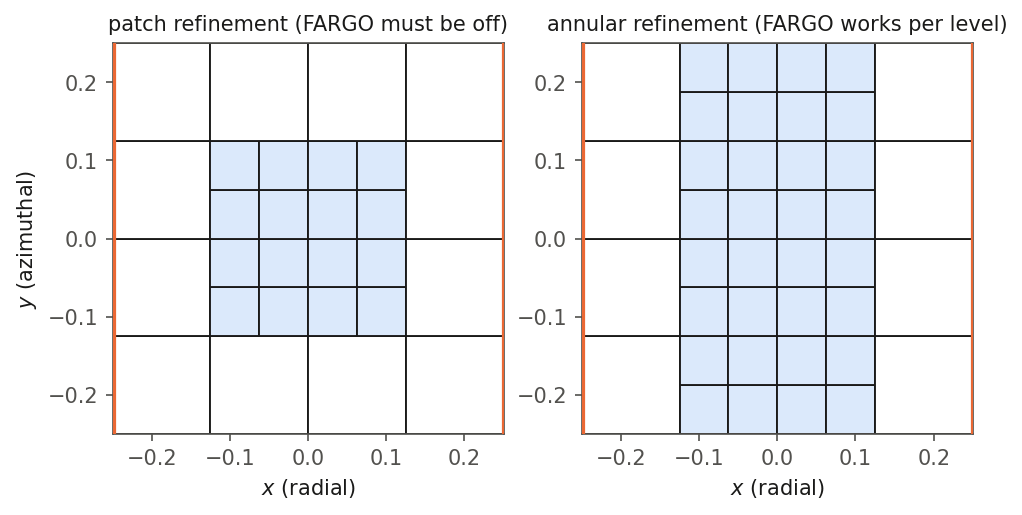
\includegraphics[width=0.78\textwidth]{figures/mg_mesh_policy.png}
  \caption{The two refinement layouts, drawn from the \code{bin} output block
  structure of actual runs (orange lines: shear-periodic $x_1$ boundaries; shaded:
  level-1 blocks). Left: a patch interior in both $x_1$ and $x_2$ --- legal only with
  \code{orbital\_advection=false}, because the coarse--fine interfaces in $y$ break
  the shift communication. Right: the annular layout --- the ring has no level jump
  in $y$, so FARGO runs per level with unmodified communication.}
  \label{fig:policy}
\end{figure}

%=======================================================================
\section{Building and compiling}
\label{sec:build}

Phase 0 needs no external dependencies beyond AthenaK's vendored Kokkos:
\begin{lstlisting}
cd athenak-multigrid
git submodule update --init kokkos     # once
mkdir build && cd build
cmake ..                               # add -D Athena_ENABLE_FFT=ON for the FFT
make -j8                               #   oracle / swing+gravity cross-checks
\end{lstlisting}
Notes: SMR/AMR runs need \code{<mesh> nghost} $\geq 4$ (even, for prolongation); the
FFT flag is only required for the tests that put gravity in the loop (it fetches
kokkos-fft and needs \code{brew install fftw} on macOS, as detailed in the companion
document). All test inputs referenced below are under \code{inputs/shearing\_box/}
and \code{inputs/tests/}; runs in this document were executed from
\code{validation/run/} and \code{validation/run\_epicycle/}.

%=======================================================================
\section{Tests and results}
\label{sec:tests}

\subsection{Frame consistency: FARGO vs.\ full-velocity, uniform grid}
\label{sec:t_nofargo}
\begin{lstlisting}
ATH=build/src/athena
$ATH -i inputs/shearing_box/hydro_incompress_shwave.athinput job/basename=shw_fargo
$ATH -i inputs/shearing_box/hydro_incompress_shwave.athinput job/basename=shw_nofargo \
     shearing_box/orbital_advection=false
# with gravity in the loop (requires FFT build):
$ATH -i inputs/tests/swing_selfgrav.athinput job/basename=SwingNoFargo \
     shearing_box/orbital_advection=false
\end{lstlisting}
The two frames agree on the frame-independent diagnostics of the JG05 vortical
shearing wave --- mass exactly, $x$-kinetic-energy history to 3.3\% (the truncation
gap between two different discretizations of the same problem). With self-gravity,
the non-FARGO swing test tracks the linearized shearing-sheet solution with
$L_2(\delta) = 1.2\times10^{-2}$ (FARGO: $0.9\times10^{-2}$) and phase-locking of the
density to the instantaneous shearing wavevector at the $10^{-12}$ level; it costs
$5.7\times$ more cycles, exactly Eq.~\eqref{eq:dtcost}.

\subsection{Refinement without FARGO (Phase 0a)}
\begin{lstlisting}
$ATH -i inputs/shearing_box/hydro_incompress_shwave_smr.athinput \
     shearing_box/orbital_advection=false
\end{lstlisting}
An interior level-1 patch (Fig.~\ref{fig:policy}, left) in the JG05 vortical-shwave
problem. The run reproduces the reference run from the original \code{test/shwave-smr}
branch \textbf{bit-for-bit} in every history column --- the port changed nothing.

\subsection{Guard checks (must abort)}
\begin{lstlisting}
# refined region snapping to a shear-boundary block: interior-x1 policy
$ATH -i inputs/shearing_box/hydro_incompress_shwave_smr.athinput \
     refined_region1/x1min=-0.24 refined_region1/x1max=-0.13
# partial-x2 ring with FARGO on: annular policy
$ATH -i inputs/shearing_box/hydro_incompress_shwave_smr.athinput \
     shearing_box/orbital_advection=true
\end{lstlisting}
Both abort with explanatory fatal errors; the second names the offending ring
(``ring at level=3 lx1=2 lx3=0 has 4 of 8 MeshBlocks'').

\subsection{FARGO on an annular ring (Phase 0b)}
\begin{lstlisting}
$ATH -i inputs/shearing_box/hydro_incompress_shwave_smr_ring.athinput \
     job/basename=ring_fargo
$ATH -i inputs/shearing_box/hydro_incompress_shwave_smr_ring.athinput \
     job/basename=ring_nofargo shearing_box/orbital_advection=false
\end{lstlisting}
The full-$x_2$ level-1 ring of Fig.~\ref{fig:policy} (right). With FARGO active on
the refined mesh: mass conserved exactly (drift $0.0$); $x$-kinetic-energy history
agrees with the non-FARGO twin to 3.8\% --- the same truncation-level gap the two
frames show on uniform grids --- and with the uniform-grid FARGO run to 4.1\%.

\subsection{Refined $x_1$ boundary faces}
\label{sec:t_bndry}
The uniform-boundary-level rule allows refinement \emph{at} the shear-periodic
boundaries when both faces are refined uniformly. The test input refines the
leftmost and rightmost root columns to level 1 over the full $x_2$/$x_3$ extent
(boundary annuli), interior at root, orbital advection on:
\begin{lstlisting}
$ATH -i inputs/shearing_box/hydro_incompress_shwave_smr_bndry.athinput
$ATH -i inputs/shearing_box/hydro_incompress_shwave_smr_bndry.athinput \
     job/basename=epi_bndry problem/ipert=1
# guard (must abort): refine only ONE face -> mixed levels across the wrap
$ATH -i inputs/shearing_box/hydro_incompress_shwave_smr_bndry.athinput \
     refined_region2/x1min=0.0 refined_region2/x1max=0.12
\end{lstlisting}
Results: the epicycle matches the analytic solution to $5.0\times10^{-6}$ ---
\emph{identical to the last digit} with the uniform-grid and interior-ring values,
so the level-1 shear-periodic wrap and the level-1 azimuthal redistribution preserve
uniform fields exactly. The vortical shwave conserves mass exactly and agrees with
the uniform run to 4.9\% in $x$-KE (interior ring: 4.1\%) and with the interior-ring
run to 0.9\%. The single-face guard aborts with a message naming the level span.

\subsection{The endurance test: epicycles for 20 orbits}
\label{sec:t_epi}
The \code{ipert=1} epicycle has spatially uniform $v_x(t)$, $v'_y(t)$: an exact
nonlinear solution that any correct $y$-shift must preserve \emph{exactly}, making it
the sharpest probe of the per-level shift and its ring-boundary communication --- any
indexing or buffer defect appears as $O(1)$ corruption. Two long runs
($L = 20$, $128^2\times4$ effective resolution, ideal EOS with
$c_s = \sqrt{5/3}$, $v_x(0) = 0.1 = 0.077\,c_s$, 20 orbits $=$ 20 epicyclic periods
since $\kappa = \Omega$ at $q = 3/2$):
\begin{lstlisting}
$ATH -i inputs/shearing_box/epicycle.athinput             # uniform 128x128x4
$ATH -i inputs/shearing_box/epicycle_smr_ring.athinput    # level-1 ring + FARGO
\end{lstlisting}

\begin{figure}[htb]
  \centering
  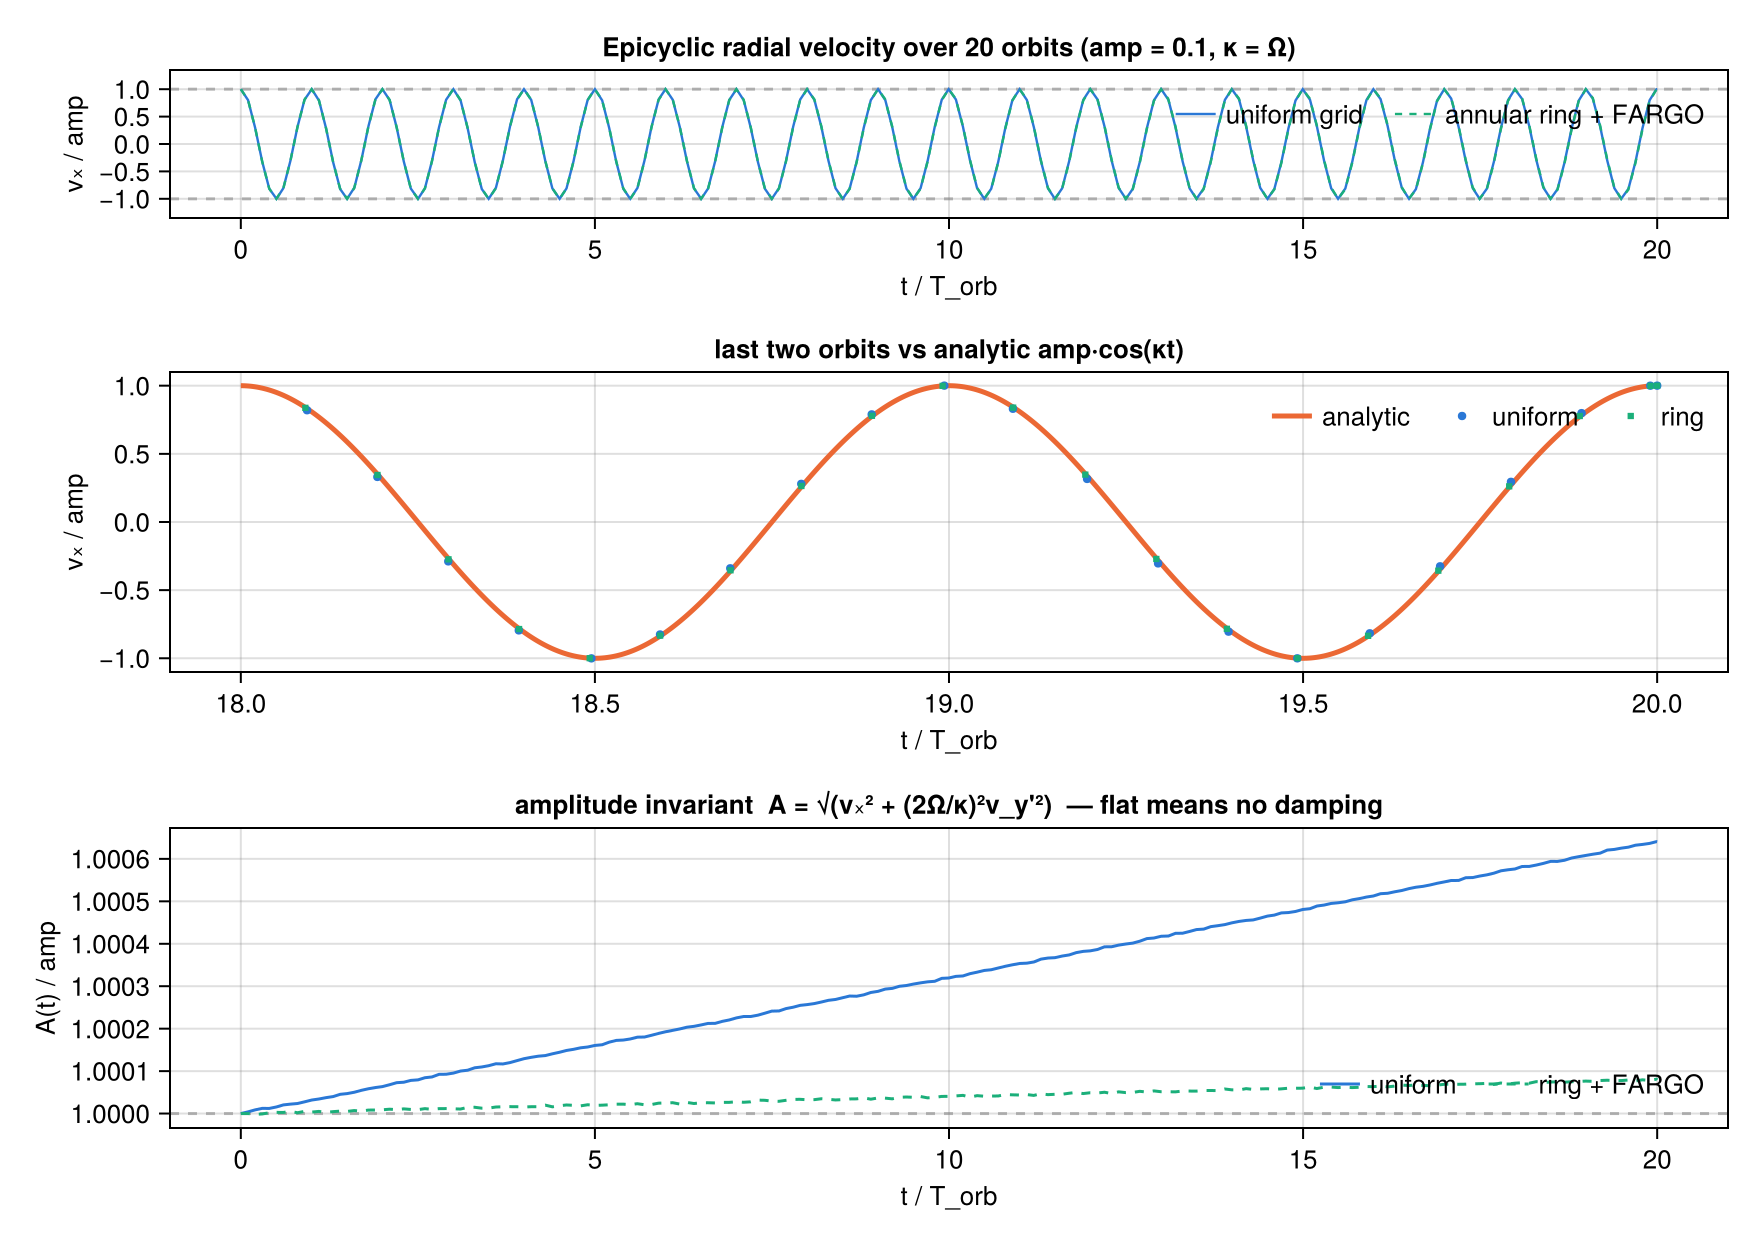
\includegraphics[width=0.95\textwidth]{figures/mg_epicycle_20orbits.png}
  \caption{Volume-averaged radial velocity of the epicycle test over 20 orbits,
  normalized to the initial amplitude. Top: both runs oscillate between $\pm1$ with
  no visible decay. Middle: the final two orbits against the analytic
  $v_x = A\cos\kappa t$. Bottom: the epicyclic amplitude invariant
  $A = [v_x^2 + (2\Omega/\kappa)^2 v_y'^2]^{1/2}$, which isolates numerical
  damping/growth from phase error.}
  \label{fig:epi20}
\end{figure}

\begin{center}
\small
\begin{tabular}{@{}lccc@{}}
\toprule
run & $v_x$ range / amp & amplitude drift, 20 orbits & max $|v_x - $analytic$|$ / amp \\
\midrule
uniform $128^2$        & $[-1.0006,\,+1.0005]$ & $+0.064\%$ & $2.4\%$ \\
annular ring $+$ FARGO & $[-1.0000,\,+1.0001]$ & $+0.008\%$ & $0.63\%$ \\
\bottomrule
\end{tabular}
\end{center}

Both runs hold the $\pm1$ envelope; the amplitude invariant is flat to a few
$\times10^{-4}$ (uniform) and $10^{-4}$ (ring) --- a slow secular \emph{growth}
characteristic of RK2 on an oscillator, not shearing-box or refinement physics. The
$3.3\%$ peak difference between the runs is pure phase drift: the ring run takes
smaller steps (finer cells) and accumulates \emph{less} RK2 phase error, which is why
the refined-mesh FARGO run is the one closer to the analytic solution. A defect in
the ring communication would instead show as amplitude noise --- none is present at
the $10^{-5}$ level.

\subsection{Summary}
\begin{center}
\small
\begin{tabular}{@{}llc@{}}
\toprule
Check & Metric & Result \\
\midrule
SMR no-FARGO vs \code{test/shwave-smr} reference & all history columns & bit-identical \\
Uniform: FARGO vs non-FARGO & mass / $x$-KE & exact / 3.3\% \\
Swing + gravity, non-FARGO vs linear theory & $L_2(\delta)$ / phase & $1.2\times10^{-2}$ / $10^{-12}$ \\
Non-FARGO cost ($L_x{=}2\pi$ box) & cycles vs FARGO & $5.7\times$, as predicted \\
Ring + FARGO: mass conservation & max drift & exact (0.0) \\
Shwave: ring-FARGO vs ring-non-FARGO & $x$-KE & 3.8\% \\
Epicycle, 20 orbits, ring + FARGO & amplitude drift / invariant & $0.008\%$ / flat to $10^{-4}$ \\
Boundary annuli + FARGO: epicycle & max rel.\ vs analytic & $5\times10^{-6}$ (= uniform) \\
Boundary annuli + FARGO: shwave & mass / $x$-KE vs uniform & exact / 4.9\% \\
Mixed-level $x_1$ boundary & --- & fatal, names the level span \\
Partial-$x_2$ ring with FARGO & --- & fatal, names the ring \\
\bottomrule
\end{tabular}
\end{center}

\noindent\textbf{Next: Phase 1} --- \code{shear\_periodic} boundary conditions in the
multigrid driver, validated against the FFT oracle (exactness at shear-periodic
instants; shearing-wave convergence order at generic phase; the swing test with
\code{solver=multigrid}), with the V-cycle convergence rate under remapped boundaries
as the quantity to watch.

\end{document}
